\chapter{Experimental Evaluation}
\label{cap:evaluation}

In this chapter the Adaptability Analyzer Software is used to study two main cases: one is the Tele Assistance System\cite{teleassist} and the other one is generated with the integrated Architecture Generator shown in Figure \ref{fig:gen-arch}

\section{Tele Assistance: A Self-Adaptive Service-Based System}
Tele Assistance System, also known as TAS, is a research, done by the University of York \cite{teleassist}, on self-adaptation in the domain of service-based systems. Originally introduced in \cite{valid-web-serv} has already been used in the evaluation of several self-adaptation solutions \cite{valid-web-serv}, \cite{sas-quant-ver}, \cite{dyn-qos-manage}, \cite{mod-evo-conf}, \cite{conq-compl}, albeit based on ad-hoc implementations, scenarios and evaluation metrics that make the comparison of these solutions and its use to evaluate other solution very difficult.

To address these limitation the University of York implemented TAS on their Research Service Platform (ReSeP) in conjunction with concrete scenarios in order to have an immediate use in evaluation of the self-adaptation solutions.

The system provides health support to chronic condition sufferers within the comfort of their homes. TAS uses a combination of sensors embedded in a wearable device and remote services from healthcare, pharmacy and emergency service providers. As shown in Figure \ref{fig:tas-workflow}, the TAS workflow takes periodical measurements of the vital parameters of a patient and employs a third-party medical service for their analysis. The analysis result may trigger the invocation of a pharmacy service to deliver new medication to the patient or to change his/her dose of medication, or the invocation of an alarm service leading, e.g., to an ambulance being dispatched to the patient. The same alarm service can be invoked directly by the patient, by using a panic button on the wearable device.

\begin{figure}[h]
	\centerline
	{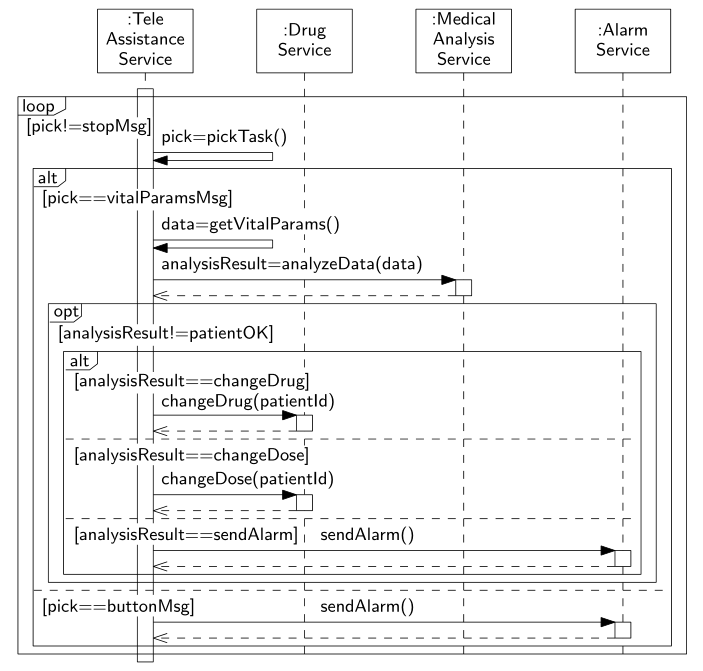
\includegraphics[scale=0.55]{img/tas-workflow.png}}
	\caption[TAS workflow]{TAS workflow}
	\label{fig:tas-workflow}
\end{figure}

They also device some generic adaptation scenarios shown in Table \ref{tab:tas-scenarios} and some metrics shown in table \ref{tab:tas-metrics}

In conclusion TAS is a reference implementation of a service based system and generic adaptation scenarios associated with different types of uncertainty. First, it aims to promote research and understanding among multiple researchers and research groups, through enabling the comparison of different self-adaptation approaches, without favouring any particular approach. Second, TAS aims to serve the advance of single research efforts by reducing the time required to evaluate self-adaptation solutions. Finally, it aims to contribute to advancing the practice of engineering self-adaptive systems, by being a realistic example of a widely used type of software system.

\begin{table}[ht!b]
	\centering
	\begin{tabular}{|l|p{3.5cm}|p{3.5cm}|p{3.5cm}|}
		\hline 
		\textbf{Scenario} & \textbf{Type of uncertainty} & \textbf{Type of adaptation} & \textbf{Type of requirements}  \\
		\hline 
		S1 & Unpredictable environment: service failure  & Switch to equivalent service; Simultaneous invocation of several services for idempotent operation & QoS: Reliability, cost \\
		\hline 
		S2 & Unpredictable environment: variation of service response time & Switch to equivalent service; Simultaneous invocation of several services for idempotent operation & QoS: Performance, cost \\
		\hline 
		S3 & Incomplete information: new service & Use new service & QoS: Reliability, performance, cost \\ 
		\hline 
		S4 & Changing requirements: new goal & Change workflow architecture; Select new service of the change on the levels & Functional: new operation \\ 
		\hline 
		S5 & Inadequate design: wrong operation sequence & Change workflow architecture & Functional: operation sequence compliance \\ 
		\hline
		
	\end{tabular} 
	\caption[TAS Scenarios]{Generic adaptation scenarios for service-based systems}
	\label{tab:tas-scenarios}
\end{table}

\begin{table}[ht!b]
	\centering
	\begin{tabular}{|p{3cm}|p{10cm}|}
		\hline 
		\textbf{Quality Attribute} & \textbf{Metrics} \\ 
		\hline 
		Reliability & Number of failed service invocations
		Number of specific operation sequence failures
		Mean time to recovery \\ 
		\hline 
		Performance & Number of specific operation sequences exceeding allowed execution time \\ 
		\hline 
		Cost & Cumulative service invocation cost over given time period \\ 
		\hline 
		Functionalities & Number of faulty process executions \\ 
		\hline 
		
	\end{tabular} 
	\caption[TAS Metrics]{Quality attributes and metrics for the evaluation and comparison of SBS self-adaptation solutions}
	\label{tab:tas-metrics}
\end{table}

\clearpage

\subsection{Adaptability Analyzer Results}

To recreate the original Tele Assistance System in the tool, the architecture has been divided in multiple components, each offering or requesting the services presented in the original system as shown in Table \ref{tab:tas-original-services}

\begin{table}[ht!b]
	\centering
	\begin{tabular}{|p{5cm}|p{3cm}|p{3cm}|}
		\hline 
		\textbf{Service Name} & \textbf{Failure Rate} & \textbf{Cost} \\ 
		\hline 
		Alarm Service 1 & 0.11 & 4.0 \\
		\hline 
		Alarm Service 2 & 0.04 & 12.0 \\ 
		\hline 
		Alarm Service 3 & 0.18 & 2.0 \\ 
		\hline 
		Medical Analysis Service 1 & 0.12 & 4.0 \\ 
		\hline
		Medical Analysis Service 2 & 0.07 & 14.0 \\ 
		\hline
		Medical Analysis Service 3 & 0.18 & 2.0 \\ 
		\hline
		Drug Service 1 & 0.01 & 5.0 \\ 
		\hline
		
	\end{tabular} 
	\caption[TAS Services]{Tele Assistance Services in the original formulation.}
	\label{tab:tas-original-services}
\end{table}

Therefore the components are divided in three main groups each offering a service between Alarm, Medical Analysis and Drug Service and one more component is added to recreate the entry point of the original system. Since the main component is not specified in the original system, I have created a plausible component with its parameters called \emph{TA}. In Table \ref{tab:tas-comp} are visible all the components and Figure \ref{fig:tas-arch} is a visual representation of the architecture generated with the tool.

\begin{table}[ht!b]
	\centering
	\begin{tabular}{|p{5cm}|p{3cm}|p{3cm}|}
		\hline 
		\textbf{Service Name} & \textbf{Availability} & \textbf{Cost} \\ 
		\hline 
		AS1 & 0.89 & 4.0 \\
		\hline 
		AS2 & 0.96 & 12.0 \\ 
		\hline 
		AS3 & 0.88 & 2.0 \\ 
		\hline 
		MAS1 & 0.88 & 4.0 \\ 
		\hline
		MAS2 & 0.93 & 14.0 \\ 
		\hline
		MAS3 & 0.82 & 2.0 \\ 
		\hline
		DS 1 & 0.99 & 5.0 \\ 
		\hline
		TA & 0.9 & 5.0 \\ 
		\hline
		
	\end{tabular} 
	\caption[TAS Components]{Tele Assistance Components as they are represented in the tool.}
	\label{tab:tas-comp}
\end{table}
In Table \ref{tab:tas-serv} are presented the components with the associated services and their parameters. Since every service is likely called as much as the other all the Required Services have a Used Probability of $ \frac{1}{3} $. All the other parameters are made up in order to make the tool work.
\begin{table}[ht!b]
	\centering
	\begin{tabular}{|p{2cm}|p{2.7cm}|p{1.7cm}|p{1.7cm}|p{1.7cm}|p{1.7cm}|}
		\hline 
		\textbf{Component} & \textbf{Service Name} & \textbf{Type of Service} & \textbf{Execution Time} & \textbf{Used Probability} & \textbf{Number of Execution per Call} \\ 
		\hline 
		AS1 & Alarm & Provided & 1.0 & & \\
		\hline 
		AS2 & Alarm & Provided & 5.0 & & \\
		\hline 
		AS3 & Alarm & Provided & 2.0 & & \\
		\hline 
		MAS1 & MedicalAnalysis & Provided & 5.0 & & \\ 
		\hline
		MAS2 & MedicalAnalysis & Provided & 10.0 & & \\ 
		\hline
		MAS3 & MedicalAnalysis & Provided & 20.0 & & \\ 
		\hline
		DS 1 & Drug & Provided & 10.0 & & \\
		\hline
		\multirow{4}{*}{TA} & Alarm & Required & & 0.33 & 1 \\
		& Drug & Required & & 0.33 & 1 \\
		& MedicalAnalysis & Required & & 0.33 & 1 \\
		& TeleAssistance & Provided & 1 & & \\
		\hline
		
	\end{tabular} 
	\caption[TAS Service]{Tele Assistance Components with their associated services.}
	\label{tab:tas-serv}
\end{table}

\begin{figure}[h]
	\centerline
	{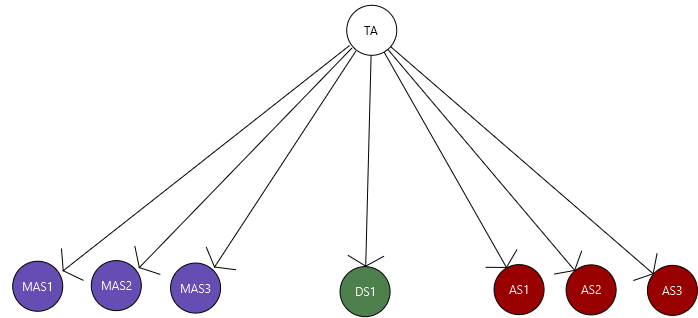
\includegraphics[scale=0.55]{img/TeleAssistance.png}}
	\caption[TAS Architecture]{TAS Architecture generated by the tool.}
	\label{fig:tas-arch}
\end{figure}

To test the architecture a workflow has been created that reflects part of the original sequence diagram shown in Figure \ref{fig:tas-workflow}. This workflow provides two cases:
\begin{itemize}
	\item The service is invoked and after having read the vital parameters and analyzed the data launches an alarm.
	\item The service is invoked and after having read the vital parameters and analyzed the data changes the drug that is currently administered to the patient.
\end{itemize}

This choice has been done since \texttt{Alt} and \texttt{Opt} blocks can't be nested in the actual implementation.

In Figure \ref{fig:tas-path1} and \ref{fig:tas-path2} are shown the two workflow in the tool.
\begin{figure}[h]
	\centerline
	{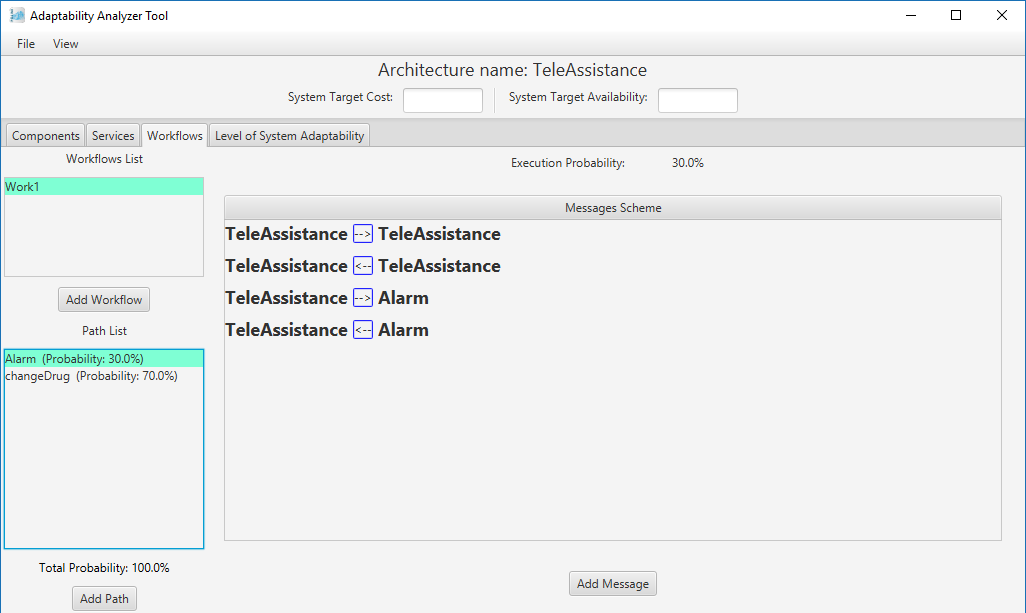
\includegraphics[scale=0.55]{img/TeleAssistancePath1.png}}
	\caption[TAS Workflow Path Alarm]{TAS workflow with the alarm path selected.}
	\label{fig:tas-path1}
\end{figure}

\begin{figure}[h]
	\centerline
	{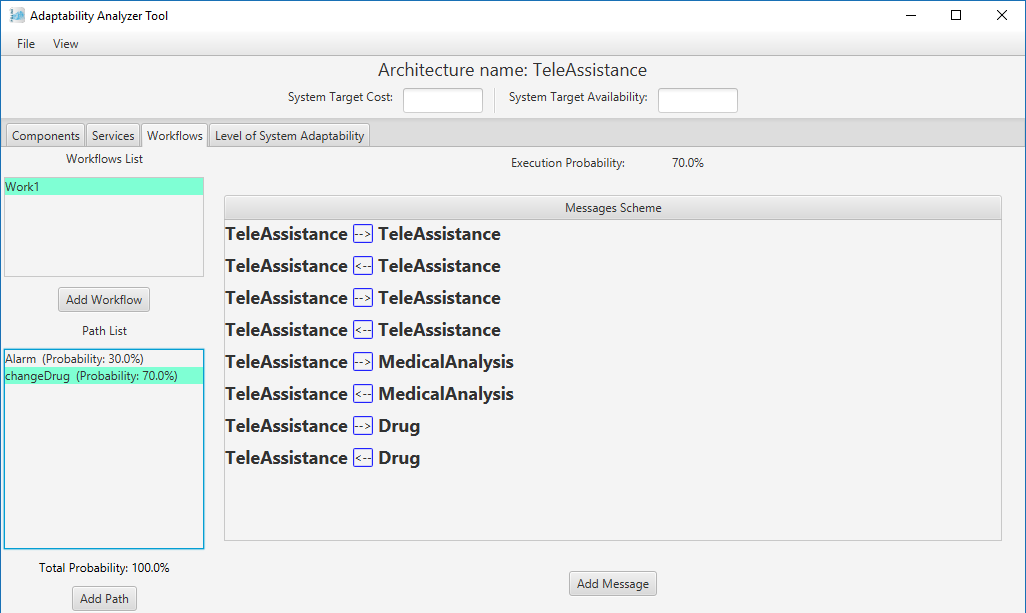
\includegraphics[scale=0.55]{img/TeleAssistancePath2.png}}
	\caption[TAS Workflow Path changeDrug]{TAS workflow with the changeDrug path selected.}
	\label{fig:tas-path2}
\end{figure}

\clearpage


